\documentclass[11pt, oneside]{article}   	% use "amsart" instead of "article" for AMSLaTeX format
\usepackage{geometry}                		% See geometry.pdf to learn the layout options. There are lots.
\geometry{letterpaper}                   		% ... or a4paper or a5paper or ... 
%\geometry{landscape}                		% Activate for rotated page geometry
%\usepackage[parfill]{parskip}    		% Activate to begin paragraphs with an empty line rather than an indent
\usepackage{graphicx}				% Use pdf, png, jpg, or eps§ with pdflatex; use eps in DVI mode
								% TeX will automatically convert eps --> pdf in pdflatex		
\usepackage{amssymb}
\usepackage{float}
%SetFonts

%SetFonts


\title{Mixed statistical and signal processing method for predictive maintenance: A use case for Ball Past Frequency Outer race detection}
\author{Yapi Donatien Achou}
%\date{}							% Activate to display a given date or no date

\begin{document}
\maketitle
\begin{figure}[H] %  figure placement: here, top, bottom, or page
   \centering
   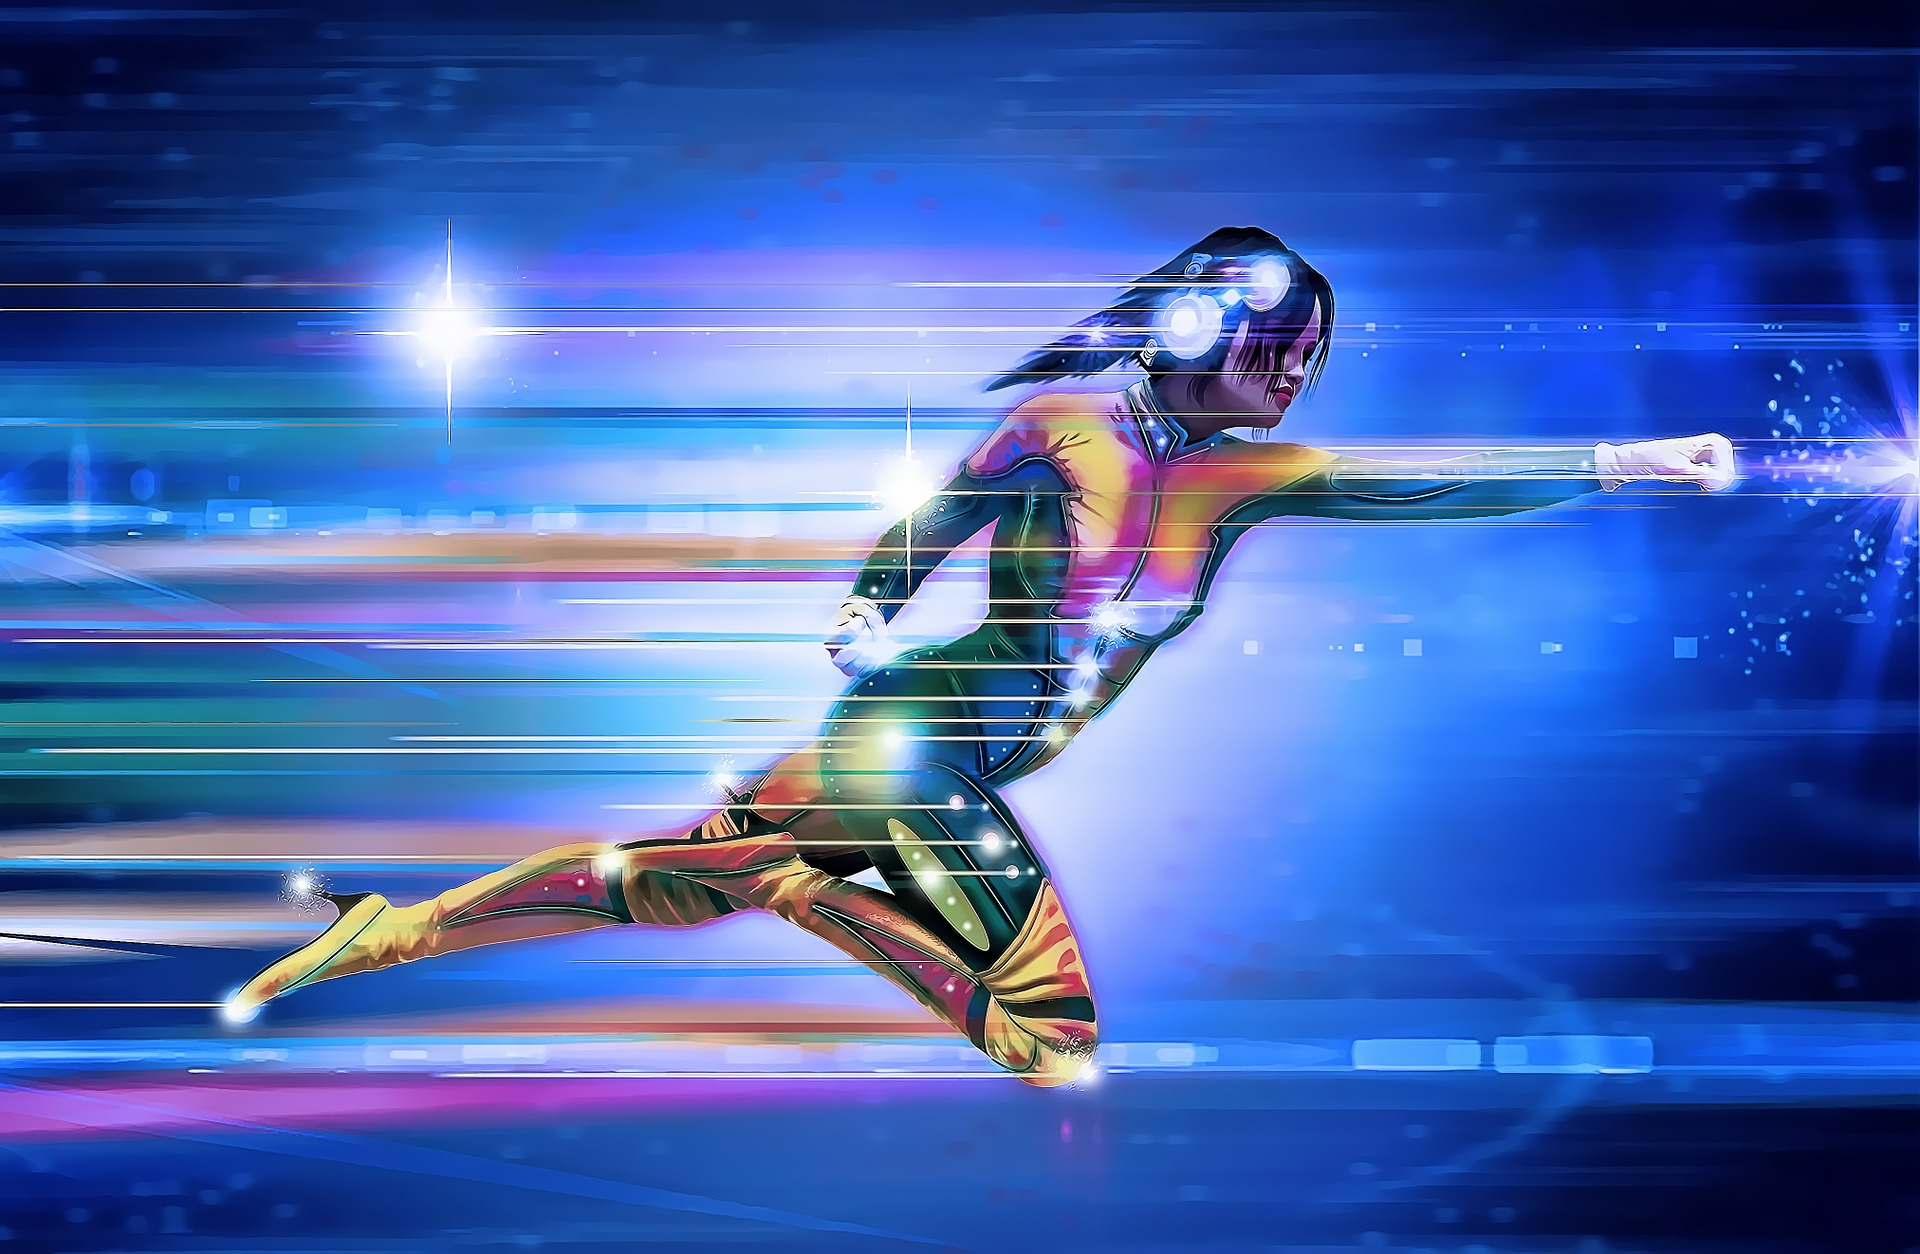
\includegraphics[width=5in]{front4} 
   \caption{}
   \label{fig:example}
\end{figure}
\section{Introduction}
Predictive maintenance can be defined as a maintenance philosophy with a set of methods used to predict and prevent machine failure in order to avoid unexpected downtime. This maintenance philosophy when correctly implemented, increases machine life time, and reduces maintenance cost [referecne].
\begin{flushleft}
In rotating machines, more then 40 $\%$ of machine malfunction can be attributed to bearing defect [references]. 
\end{flushleft}
\begin{figure}[H] %  figure placement: here, top, bottom, or page
   \centering
   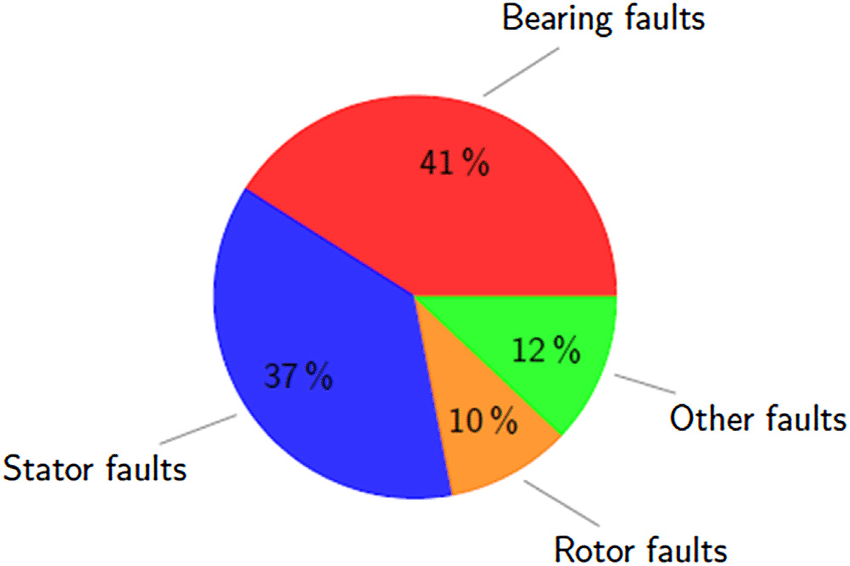
\includegraphics[width=5in]{pie.png} 
   \caption{Defect statistic, taken from [reference]}
   \label{fig:pie}
\end{figure}
In this article I will present a mixed method, a statistical approach and  a purely signal processing method to detect bearing defect.

\section{Defining the use case}
\begin{figure}[H] %  figure placement: here, top, bottom, or page
   \centering
   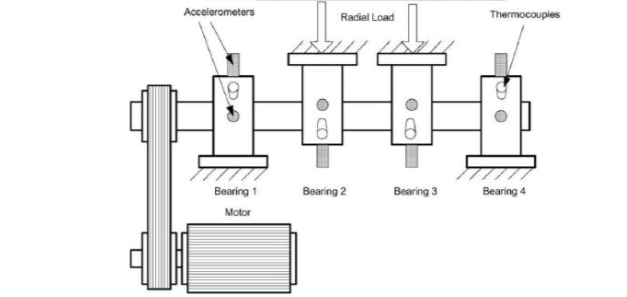
\includegraphics[width=4in]{experiment} 
   \caption{Experimental set up}
   \label{fig:exp}
\end{figure}
The data used in this use case was generated by the Intelligence Maintenance system (IMS) [link to the IMS].
Three separate experiments involving four bearings were performed on a motor. The motor shaft is kept at 2000 RPM.
There are 984 samples where each sample represents a 1-second vibration signal snapshots recorded every 10 minutes.
Each sample consists of 20 480 data points with sampling rate of 20 000 Hz.
In this article we will be using the second experiment. At the end of the experiment outer race failure occurred in bearing 1.




\section{Signal processing approach}
\begin{figure}[H] %  figure placement: here, top, bottom, or page
   \centering
   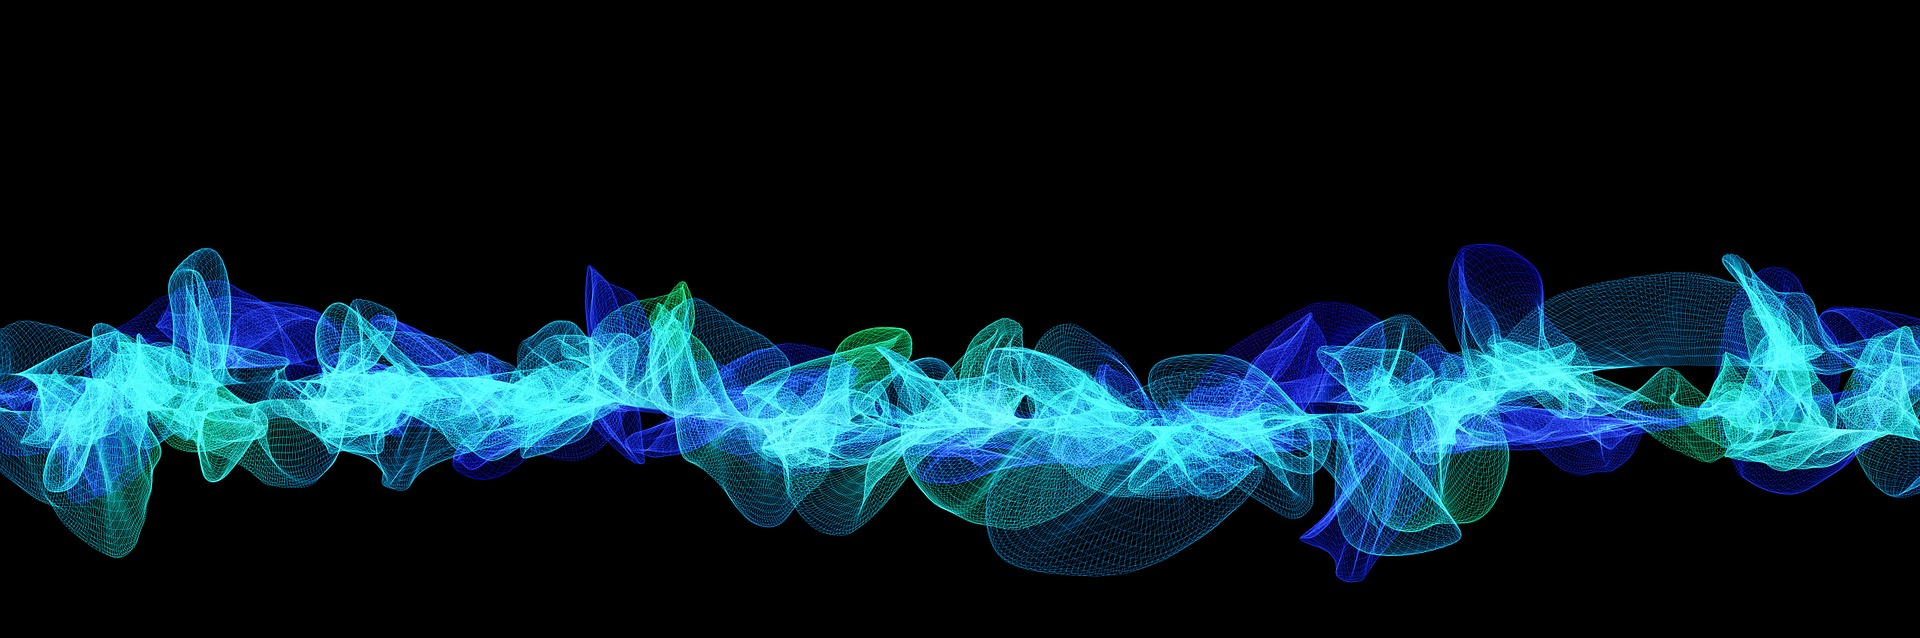
\includegraphics[width=4in]{vibration} 
   \caption{}
   \label{fig:example}
\end{figure}
Inn this approach we use the old goody Fourier transform. Firstly, we need the defect frequency for the outer race defect. The bearing type used are Rexnor ZA-2115 type with a defect frequency of 0.1182. To find the defect frequency in Hz we multiply 0.1182 by the RPM (2000), which is 236.4 Hz. Note that the defect frequency is computed from the geometry of the bearing 
\begin{figure}[htbp] %  figure placement: here, top, bottom, or page
   \centering
   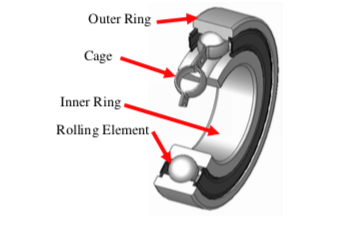
\includegraphics[width=4in]{bearing.png} 
   \caption{}
   \label{fig:example}
\end{figure}
\begin{flushleft}
Next, we compute the envelop spectrum for each vibration signal from FFT (Fast Fourier Transform). The envelop spectrum is used to detect early sign of failure. Recall that a vibration signal can be decomposed into its sub components, where each  sub component 
is characterised by its frequency and its amplitude. Early sign of failure are represented by a low amplitude and hight frequency sub component of the vibration original signal.
\end{flushleft}

%\begin{figure}[H] %  figure placement: here, top, bottom, or page
%   \centering
%   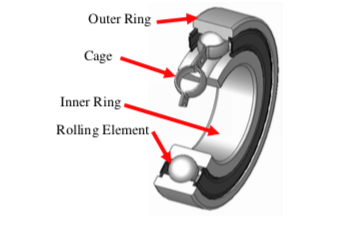
\includegraphics[width=4in]{bearing.png} 
%   \caption{Geometrical representation of a ball bearing (Figure taken form [32])}
%   \label{fig:bearing}
%\end{figure}

\section{Statistical approach: dissimilarity measure}

\section{Mixed method: statistical and wavelet aproach}

\section{Comparison}



\end{document}  